\chapter{CONCLUSÃO}
\label{cap:conclusao}

Toda minha experiência no Laboratório foi excepcional e de grande valia a meu desenvolvimento profissional e pessoal, aprendendo a lidar com diversos problemas e pessoas.
Quando iniciei o estágio, meu conhecimento era somente relacionado ao contexto acadêmico lecionado pela universidade até o quinto período de graduação, o que em sua grande maioria eram conhecimentos e teorias sobre otimizações e códigos de baixo nível.
Após alguns meses como estagiário, já possuía propriedade intelectual e autoridade para opinar em decisões estruturais de projetos, tecnologias e até mesmo estabelecer prazos, obviamente após inúmeros erros e muito estudo.
 
Os profissionais quais tive o prazer de trabalhar sempre foram muito agradáveis, solícitos e agregaram muito valor em meu desenvolvimento.

Devido aos problemas superados e projetos desenvolvidos no LEMAF, fui capaz de desenvolver minhas habilidades como desenvolvedor web e criar grande portfólio, abrindo diversas portas para o mercado de trabalho.
O estágio também me proporcionou uma visão abrangente de cargos e caminhos que poderia trilhar dentro da minha área de estudo, o que fez aumentar minhas oportunidades de escolhas e afirmar o que eu realmente tinha como desejo e vocação: ser desenvolvedor.

Posso afirmar que, os principais motivos da contratação em meu atual emprego na empresa Equals, foram minhas experiências com as tecnologias ReactJS, Spring e principalmente o desenvolvimento do Cria Design.

\begin{figure}[H]
\centering
\caption{Bilhete recebido da confraternização no fim de 2018} %legenda

\includegraphics[scale=0.3]{agradecimento}\\  % o 0.9 indica 90% do tamanho original
% pdfLaTeX aceita figuras no formato PNG, JPG ou PDF
% figuras vetoriais podem ser exportadas para eps e depois convertidas para pdf usando epstopdf
\label{fig:exemplo} %rotulo para refencia
\end{figure}

Toda minha trajetória no laboratório foi muito prazerosa e produtiva. No meu ultimo dia de estágio, fui convidado a participar do podcast da empresa, onde compartilhei um pouco da minha experiência com os outros funcionários \footnote{\url{http://blog.ti.lemaf.ufla.br/2019/08/22/podcast-5/}}.

\begin{figure}[H]
\centering
\caption{Convenção Lemaf / Fundecc 2018} %legenda
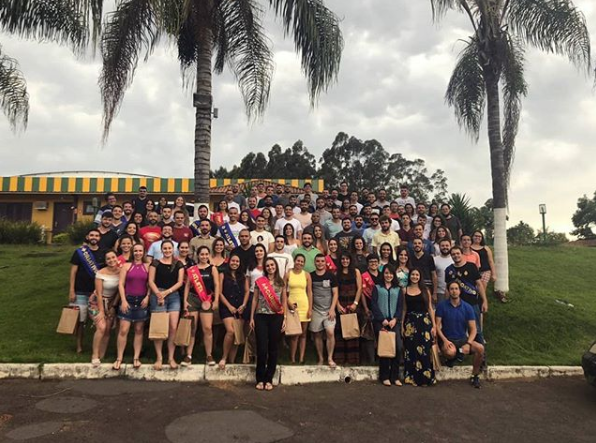
\includegraphics[scale=1]{convensao}\\  % o 0.9 indica 90% do tamanho original
% pdfLaTeX aceita figuras no formato PNG, JPG ou PDF
% figuras vetoriais podem ser exportadas para eps e depois convertidas para pdf usando epstopdf
{\small Fonte: https://www.instagram.com/p/Brlf2IKlAmi/} %Fonte da imagem
\label{fig:exemplo} %rotulo para refencia
\end{figure}
    